The Kernel Polynomial Method (KPM) is a powerful technique for approximating spectral properties of large matrices \cite{weisse2006,linsaadyang14}. It employs polynomial expansions to efficiently estimate quantities such as the spectral density and related functions. We previously motivated the replacement of the Dirac delta distribution with a regular function~$f$, and now use the variant of KPM that incorporates this regularization using Chebyshev polynomials.
The coefficients of the polynomials are derived from the method of moments, in order to obtain an estimator function as in statistics.

\section{Basic properties of Chebyshev polynomials}
Among the possible choices, Chebyshev polynomials of the first kind are particularly well-suited due to their favorable mathematical properties, which we will outline below. We note that these properties are not unique, as Legendre polynomials or Hermite polynomials are examples of other good candidates.

First, let's look how Chebyshev polynomials are defined.
Using the trigonometric functions, they can be expressed as follows:

\[ T_k(x) =
\begin{cases}

\cos(k \arccos(x))                & \quad \text{for } k \in [-1, 1],\\
    \cosh(k \arcosh(x))           & \quad \text{for } k > 1,\\
    (-1)^k \cosh(k \arcosh(-x))   & \quad \text{for } k < -1.
\end{cases}
\]

For simplicity, we only want to use the formula $T_k(x) = \cos(k \arccos(x))$.
This means to only consider matrices that have eigenvalues within the intervall $[-1, 1]$.
In the case that this condition should not be fulfilled, the eigenvalues can be transformed accordingly.

For this, let $\lambda_{lb}$ and $\lambda_{ub}$ be the lower and upper bound for the eigenvalues of $A$, respectively.
To find these, well-established methods like the Gershgorin circle theorem can be used.

Define
\[
c := \frac{\lambda_{lb} + \lambda_{ub}}{2} \quad \text{and} \quad d := \frac{\lambda_{ub} - \lambda_{lb}}{2}
\]
Then, the matrix $B = \frac{A - c*I_n}{d}$ has eigenvalues in the interval $[-1, 1]$.
A visualization of this is linked in the appendix.

Another way to define Chebyshev polynomials is by calculating them using the recursion formula
\[
T_{k}(x) = 2xT_{k - 1}(x) - T_{k - 2}(x),
\]
where the starting conditions are given by $T_0(x) = 1$ and $T_1(x) = x$.

Let's recall that for a given interval~$[a, b]$ and weight function~$w(x) \geq 0$ defined on that interval, we define the inner product
\[
\langle f, g \rangle_w := \int\limits_a^b w(x) f(x) g(x) \dx.
\]
Now, let
\[
h(x) := \frac{1}{\sqrt{1 - x^2}}
\]
be a weight function on $[-1, 1]$. We investigate the inner product of two Chebyshev polynomials with respect to this weight function:

\begin{lemma}[Orthogonality of Chebyshev Polynomials]
Let $T_k(x)$ denote the Chebyshev polynomials, and let $h(x) = \frac{1}{\sqrt{1 - x^2}}$ be the weight function on $[-1, 1]$. Then, for all integers $k, l \geq 0$,
\begin{equation} \label{eq:orthogonality}
    \int\limits_{-1}^1 \frac{1}{\sqrt{1 - x^2}} T_k(x) T_l(x) \dx =
    \begin{cases}
        0               & \text{if } k \neq l,\\
        \pi             & \text{if } k = l = 0,\\
        \frac{\pi}{2}   & \text{if } k = l \neq 0.
    \end{cases}
\end{equation}
\end{lemma}

\begin{proof}
Recall that $T_k(x) = \cos(k \arccos(x))$ for $x \in [-1, 1]$. Let $x = \cos \theta$ with $\theta \in [0, \pi]$. Then $\dx = -\sin \theta \, d\theta$ and $\sqrt{1 - x^2} = \sin \theta$.

Substituting, we have:
\begin{align*}
    \int\limits_{-1}^1 \frac{1}{\sqrt{1 - x^2}} T_k(x) T_l(x) \dx
    &= \int\limits_{\theta=\pi}^{0} \frac{1}{\sin \theta} \cos(k \theta) \cos(l \theta) (-\sin \theta) d\theta \\
    &= \int\limits_{0}^{\pi} \cos(k \theta) \cos(l \theta) d\theta
\end{align*}

The orthogonality of cosine functions on $[0, \pi]$ gives:
\begin{align*}
    \int\limits_{0}^{\pi} \cos(k \theta) \cos(l \theta) d\theta =
    \begin{cases}
        0               & \text{if } k \neq l,\\
        \pi             & \text{if } k = l = 0,\\
        \frac{\pi}{2}   & \text{if } k = l \neq 0.
    \end{cases}
\end{align*}
which proves the lemma.
\end{proof}

\section{Approximating the spectral density}
We now define the $\hat{\phi}$ as the product of spectral density with the inverse of the weight function~$h(x)$:
\[
\hat{\phi}(x) := \sqrt{1 - x^2} \phi(x) = \sqrt{1 - x^2} \, \cdot \, \frac{1}{n} \sum_{j = 1}^n \delta(x - \lambda_j)
\]
Let $g \in \SR$, the Schwartz space defined in Definition \ref{def:Schwartz space}, and let $\mu_k~\in~\R$ coefficients to be determined such that the following equation holds:

\[
    \int \limits_{-1}^1 \hat{\phi}(x) g(x) \dx = \int \limits_{-1}^1 \sum_{k = 0}^{\infty} \mu_k T_k(x) g(x) \dx
\]

If this is true for arbitrary $g \in \SR$, we can simplify the equation above to

\begin{equation} \label{eq:Chebyshev-Expansion}
    \hat{\phi}(x) = \sum_{k = 0}^{\infty} \mu_k T_k(x)
\end{equation}


Now utilize the orthogonality of the Chebyshev polynomials to calculate a specific coefficient~$\mu_k$.
Note that~$\delta_{k0}$ in this context denotes the Kronecker delta, and therefore equals $1$ for~$k = 0$ and $0$ for~$k \neq 0$. Applying the inner product defined above to both sides of the equation yields

\begin{align*}
    & \; \; \left \langle \sum_{l = 0}^{\infty} \mu_l T_l(x), T_k(x) \right \rangle_h = \left \langle \hat{\phi}(x), T_k(x) \right \rangle_h \\
    \implies & \int\limits_{-1}^1 \frac{1}{\sqrt{1 - x^2}} \left(\sum_{l = 0}^{\infty} \mu_l T_l(x)\right) T_k(x) \dx = \int\limits_{-1}^1 \frac{1}{\sqrt{1 - x^2}} \hat{\phi}(x) T_k(x) \dx.\\
\end{align*}

On the left side, every term of the sum except for the~$k$-th term vanishes due to the orthogonality of the Chebyshev polynomials, while we make use of our definition of~$\hat{\phi}$ on the right side. Therefore, we have

\[
    \mu_k \frac{\pi}{2 - \delta_{k0}} = \int\limits_{-1}^1 \frac{1}{\sqrt{1 - x^2}} \sqrt{1 - x^2} \phi(x) T_k(x) \dx \implies \mu_k = \frac{2 - \delta_{k0}}{\pi} \int\limits_{-1}^1 \phi(x) T_k(x) \dx
\]

By applying the Dirac delta distribution we obtain:
\begin{align*}
    \mu_k = \frac{2 - \delta_{k0}}{\pi} \int\limits_{-1}^1 \phi(t) T_k(t) \dt &= \frac{2 - \delta_{k0}}{\pi} \int\limits_{-1}^1 \frac{1}{n} \sum_{j = 1}^n \delta(t - \lambda_j) T_k(t) \dt \\
    &= \frac{2 - \delta_{k0}}{n \pi} \sum_{j = 1}^n T_k(\lambda_j)\\
    &= \frac{2 - \delta_{k0}}{n \pi} \Tr(T_k(A))
\end{align*}

with $\Tr(T_k(A)) := \displaystyle \sum_{j = 1}^n T_k(\lambda_j)$ the \emph{trace} of the Chebyshev polynomial applied to the matrix $A$. This means we are in need of an estimator for $\Tr(T_k(A))$.

\section{Estimating the trace of Chebyshev polynomials}

We want to obtain the corollary of the following generalized theorem:

\begin{theorem}
    Let $A \in \C^{n \times n}$ be a normal matrix with spectral decomposition
    \[
    A = U \Lambda U^* \quad \text{where} \quad UU^* = I_n \text{ and } \Lambda = \diag(\lambda_1, ..., \lambda_n)
    \]
    Let $\beta, v \in \C^n$ with $v = U\beta$.
    Suppose $v$ is a random vector whose entries $v_i$ are independent and identically distributed standard complex normal variables,
    i.e., $v_i \sim_\text{i.i.d.} \mathcal{N}_\C(0, 1)$, meaning $\Real(v_i), \Imag(v_i)$ are independent $\mathcal{N}(0, \frac{1}{2})$.
    Then
    \begin{equation} \label{eq:complex_normal_vector}
        \E[v] = 0 \quad \text{and} \quad \E[v v^*] = I_n,
    \end{equation}
    and it follows that
    \[
    \E[\beta] = 0 \quad \text{and} \quad \E[\beta \beta^*] = I_n.
    \]
\end{theorem}


\begin{proof}[Proof]
    Since the expectation operator is linear, it holds that
    \[
    \E[v] = \E[U\beta] = U\E[\beta] = 0 \implies \E[\beta] = 0
    \]
    Furthermore it holds that
    \[
    I_n = \E[vv^*] = \E[(U\beta)(U\beta)^*] = \E[U\beta \beta^*U^*] = U \E[\beta \beta^*]U^*
    \]
    Multiplying both sides with $U^*$ and $U$ yields:
    \[
    U^* I_n U = U^* U \E[\beta \beta^*]U^* U = \E[\beta \beta^*]
    \]
    Since $U$ is unitary, we have shown that $\E[\beta \beta^*] = I_n$.
\end{proof}

This theorem has a nice corollary when investigating a matrix function $f(A)$.
In that case,
\begin{align*}
    \E\left[v^* f(A) v\right] = \E\left[(U\beta)^* f(U\Lambda U^*) (U\beta)\right] &= \E\left[\beta^* U^* U f(\Lambda) U^* U \beta\right] \\
    &= \E\left[\beta^* f(\Lambda) \beta\right] \\
    &= \E\left[\sum_{j = 1}^n |\beta_j|^2 f(\lambda_j) \right] \\
    &= \sum_{j = 1}^n f(\lambda_j) \E\left[ |\beta_j|^2 \right] \\
    &= \sum_{j = 1}^n f(\lambda_j)
\end{align*}

or, more concisely,
\[
    \E\left[v^* f(A) v\right] = \Tr(f(A)).
\]

We now have a method to calculate the trace of a matrix function $f(A)$,
using only vector multiplications with $A$.

\section{The Kernel Polynomial Method algorithm}

Now let $n_{\text{vec}} \in \N$ and consider random vectors $v_0^{(1)}, v_0^{(2)}, \dots, v_0^{(n_{\text{vec}})}$,
each drawn independently from the standard normal distribution, that is, $\mathbb{E}[v_0^{(k)}] = 0$ and $\mathbb{E}\left[v_0^{(k)} \left(v_0^{(k)}\right)^T\right] = I_n$.
It follows from $\E\left[v^* f(A) v\right] = \Tr(f(A))$ that
\[
\zeta_k = \frac{1}{n_{\text{vec}}} \sum_{l = 1}^{n_{\text{vec}}} \left( v_0^{(l)} \right)^T T_k(A) v_0^{(l)}
\]
is a good estimator for $\Tr(T_k(A))$ and therefore
\[
\mu_k \approx \frac{2 - \delta_{k0}}{n \pi} \zeta_k.
\]

In order to determine the $\zeta_k$, let $v_0 \equiv v_0^{(l)}$.
Using the recursion formula for Chebyschev polynomials, we can calculate
\[
T_{k + 1}(A)v_0 = 2 A T_k(A) v_0 - T_{k - 1}(A) v_0.
\]
For $v_k \equiv T_k(A)v_0$ it also holds that
\[
v_{k + 1} = 2 A v_k - v_{k - 1}.
\]

With this we are fully equipped for the final calculation and the goal of the KPM is reached:
Instead of having to multiply matrices with other matrices, it now suffices to multiply matrices with vectors.
Now we can approximate $\phi(x)$ as closely as we like.
As aforementioned, it is not always desirable to have an infinitely exact approximation.
Since it holds that
\[
\lim \limits_{k \to \infty} \mu_k \to 0
\]
and we are only interested in $T_k(x)$ with $k \leq M$.
Therefore we estimate $\phi$ with
\begin{equation} \label{Approximated spectral density}
    \tilde{\phi}_M(x) = \frac{1}{\sqrt{1 - x^2}} \sum_{k = 0}^{M} \mu_k T_k(x)
\end{equation}
The following pseudo code is based on \cite[p.~10]{linsaadyang14} and summarizes the steps described above.
The implementation is done in Python, and linked in the appendix.

\begin{algorithm}
    \caption{The Kernel Polynomial Method}\label{alg:cap}
    \begin{algorithmic}[5]
    \Require $A = A^* \in \mathbb{C}^{n \times n}$ with eigenvalues in the intervall $[-1, 1]$
    \Ensure Estimated spectral density \{$\tilde{\phi}_M(t_i)$\}\\
    \For{$k = 0 : M$}
    \State $\zeta_k \gets 0$
    \EndFor
    \For{$l = 1 : n_{\text{vec}}$}
    \State $\text{Choose a random new vector } v_0^{(l)}\text{;}$ \Comment{$v_{0_i}^{(l)} \sim_\text{ i.i.d. } \mathcal{N}(0, 1)$}
    \For{$k = 0 : M$}
    \State $\text{Calculate } \zeta_k \gets \zeta_k + \left( v_0^{(l)} \right)^T v_k{(l)}\text{;}$  
    \If{$k = 0$}
    \State $v_1^{(l)} \gets A v_0^{(l)}$
    \Else
    \State $v_{k+1}^{(l)} \gets 2 A v_k^{(l)} - v_{k-1}^{(l)}$ \Comment{Three term recursion}
    \EndIf
    \EndFor
    \EndFor
    \For{$k = 0 : M$}
    \State $\zeta_k \gets \frac{\zeta_k}{n_{\text{vec}}}$
    \State $\mu_k \gets \frac{2 - \delta_{k0}}{n \pi} \zeta_k$
    \EndFor
    \State $\text{Evaluate } \tilde{\phi}_M(t_i) \eqref{Approximated spectral density}$
    \end{algorithmic}
\end{algorithm}

Applying the Cayley transform to an arbitrary unitary matrix $U$ yields a Hermitian matrix $H$;
and as this is the case, the KPM can be applied to unitary matrices as well.

\section{The Choice of Random Unitary Matrices}

When generating random unitary matrices for numerical experiments,
it is important to ensure that their eigenvalues are distributed uniformly on the unit circle,
as predicted by random matrix theory~\cite{mezzadri2007}.
A common approach is to generate a random complex matrix $A$ with independent standard normal entries
and then construct a unitary matrix from $A$ using either the QR decomposition or the singular value decomposition (SVD).
In the QR approach, $A$ is factored as $A = QR$, where $Q$ is unitary and $R$ is upper triangular.
The matrix $Q$ is then used as the random unitary matrix.
In the SVD approach, $A$ is factored as $A = U \Sigma V^*$,
and either $U$ or $V$ (both unitary) can be used as a random unitary matrix.
Although both methods produce unitary matrices, their statistical properties differ.
The SVD-based approach yields unitary matrices whose eigenvalues are uniformly distributed on the unit circle,
matching the theoretical prediction for random unitary matrices (the so-called Haar measure)~\cite{mezzadri2007}.
In contrast, the QR-based approach does not generally produce a uniform distribution of eigenvalues on the unit circle.
This distinction is important for applications where the spectral properties of random unitary matrices play a central role,
such as in the study of spectral densities.
For such purposes, the SVD-based construction is preferable,
as it ensures the correct statistical behavior of the eigenvalues.

\begin{figure}[htb]
    \centering
    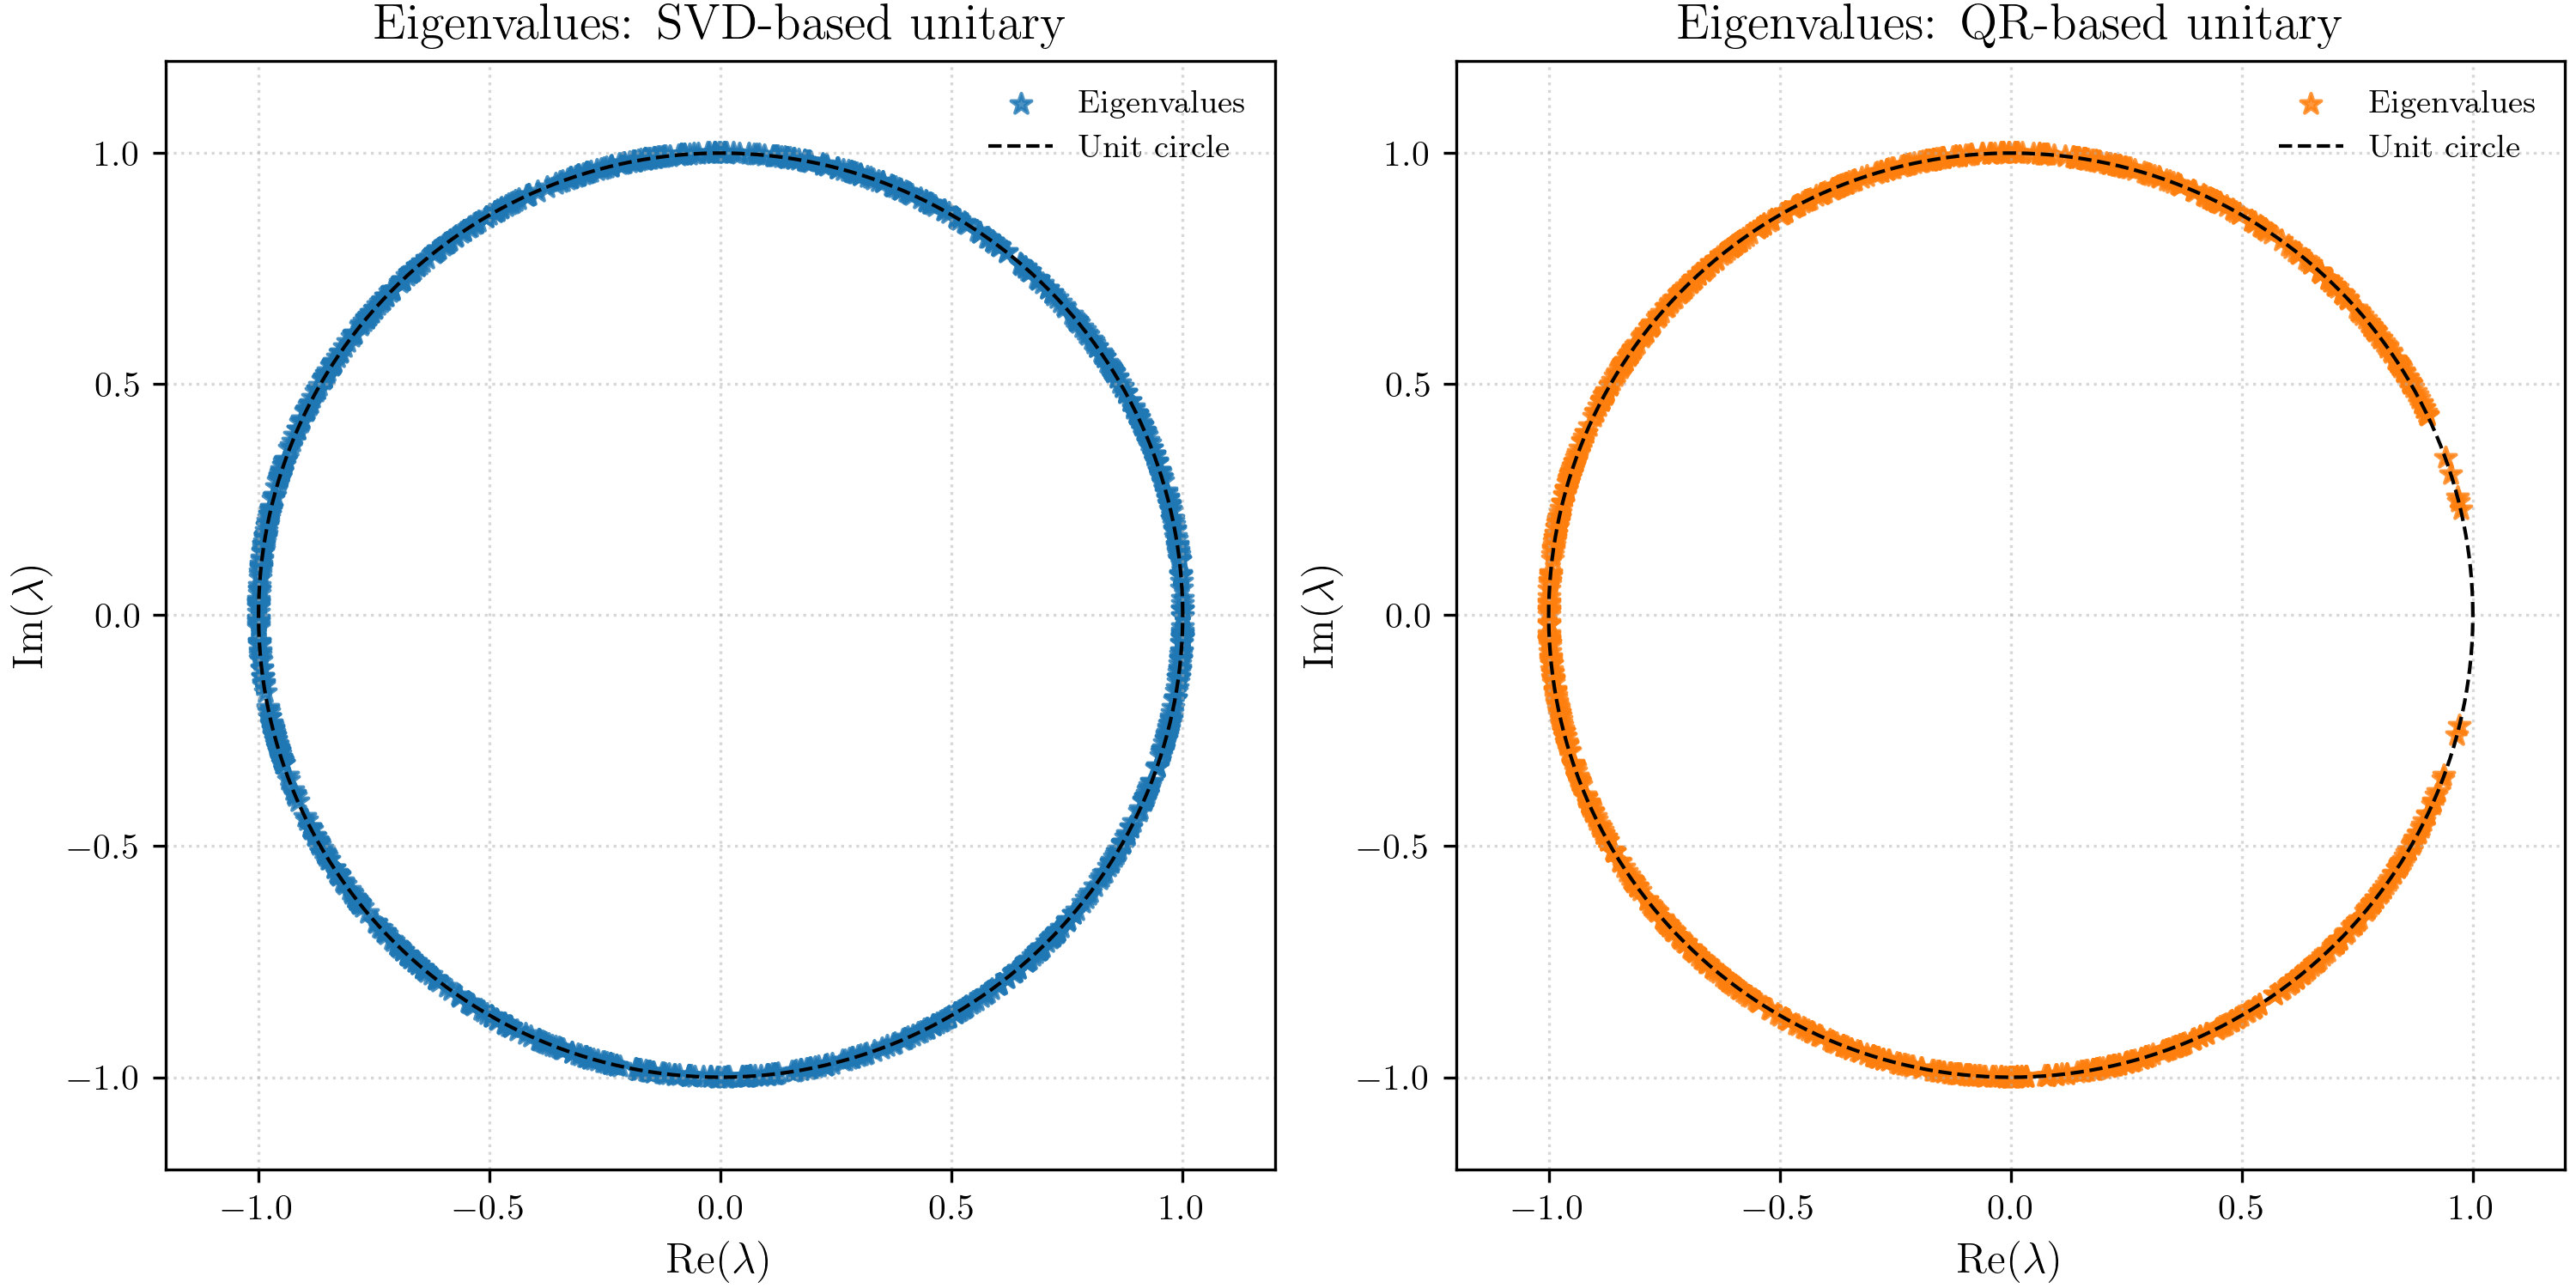
\includegraphics[width=1\textwidth]{Graphics/eigenvalue_comparison.png}
    \caption{Eigenvalue distributions of random unitary matrices generated via SVD and QR.}
    \label{fig:eigenvalue-comparison}
\end{figure}